\documentclass[final, dvipdfmx]{beamer}
\usepackage[
	orientation=portrait,
	size=a0paper,
	scale=1.4,
	debug
	]{beamerposter}
\mode<presentation>{
	\usetheme{singapore}
	\useoutertheme{infolines}
	\usecolortheme{rose} % いじらない
	\usefonttheme{professionalfonts}
	\useinnertheme{rectangles}
	\useoutertheme{tree}
}
% 日本語(非英語)に対応
\usepackage[japanese]{babel}
% ポスターで不要な要素の非表示
\setbeamertemplate{navigation symbols}{}
\setbeamertemplate{headline}{}
\setbeamertemplate{footline}{}
% 日本語をゴシック体
\renewcommand{\kanjifamilydefault}{\gtdefault}
% blockの色の設定
%\setbeamercolor{block body}{bg=white, fg=black} % tcbsetforeverylayer とかでやったほうがいいかも
% フォントの設定
%\usefonttheme[onlymath]{serif}
%\setbeamerfont{caption}{size=\normalsize}
\setbeamerfont{block title}{size=\LARGE}
%\setbeamerfont*{itemize/enumerate body}{size=\large}
%\setbeamerfont*{itemize/enumerate subbody}{parent=itemize/enumerate body, size=\large}
%\setbeamerfont*{itemize/enumerate subsubbody}{parent=itemize/enumerate subbody, size=\large}
% 箇条書きのアイコンを変更
\setbeamertemplate{itemize item}[circle]
\setbeamertemplate{enumerate items}[default]
\setbeamertemplate{itemize subitem}[triangle]
%\setbeamercolor{enumerate item}{fg=black}
% 参考文献のアイコンを標準のに
\setbeamertemplate{bibliography item}[text]
% 参考文献の文字色を変更
\setbeamercolor*{bibliography item}{fg=black}
\setbeamercolor*{bibliography entry author}{fg=black}
\setbeamercolor*{bibliography entry title}{fg=black}
\setbeamercolor*{bibliography entry location}{fg=black}
% Beamer-blockの実装をtcolorboxで行う、TeX Live 2024が必要
\useinnertheme[rounded]{tcolorbox}
\tcbsetforeverylayer{
  frame style={draw=block title.bg, line width=4mm}
}

% 数式
\usepackage{amsmath}
\usepackage{amssymb}
\usepackage{physics}
\usepackage{mathtools}
% 行列の表現を拡張する、まだよくわかっていない
\usepackage{nicematrix}
% 画像・表
\usepackage{graphicx}
\usepackage{color}
\usepackage{here}
% 図表のcaptionを設定
\usepackage{caption}
\usepackage[subrefformat=parens]{subcaption}
\captionsetup[figure]{name=図}
\captionsetup[table]{name=表}
\setbeamertemplate{caption}[numbered]
% 疑似コード
\usepackage{algorithm}
\usepackage{algpseudocode}
\algnewcommand{\IIf}[1]{\State\algorithmicif\ #1\ \algorithmicthen}
\algnewcommand{\EndIIf}{\unskip\ \algorithmicend\ \algorithmicif}
% 画像フォルダへのパスを追加
\graphicspath{ {fig/} }
% タイトルの背景に色を付けるために使用
\usepackage{tcolorbox}
% コメントアウト
\usepackage{comment}
% ダミーテキスト
\usepackage{lipsum}
% PDFのメタ情報・URL
\usepackage{hyperref}
\usepackage{pxjahyper}
\hypersetup{
	setpagesize=false,
	bookmarks=true,
	bookmarksdepth=tocdepth,
	bookmarksnumbered=true,
	hidelinks,
	hyperfootnotes=false,
	pdftitle={一般化シフト線形方程式に対するMINRES法の適用と性能評価},
	pdfsubject={第22回計算数学研究会},
	pdfauthor={日高 俊太郎},
	pdfkeywords={シフト線形方程式, Krylov部分空間法, MINRES法, 一般化固有値問題}
}

% コマンドの設定
\newcommand{\equref}[1]{(\ref{#1})}					% 括弧で囲まれた参照
\newcommand{\Equref}[1]{式(\ref{#1})}				% 数式の参照
\newcommand{\Tabref}[1]{表\ref{#1}}					% 表の参照
\newcommand{\Figref}[1]{図\ref{#1}}					% 図の参照
\renewcommand{\top}[0]{\mathrm{T}}					% 転置
\newcommand{\htop}[0]{\mathrm{H}}					% Hermite転置
\renewcommand{\i}[0]{\mathrm{i}}					% 虚数単位
\newcommand{\KS}[3]{\mathcal{K}_{#1}({#2}, {#3})}			% Krylov Subspace
\newcommand{\inpro}[2]{\langle #1, #2 \rangle}			% 内積
\newcommand{\conj}[1]{\overline{#1}}					% 複素共役
% itemizeのシンボルをitemize外で使えるようにする
% https://tex.stackexchange.com/questions/519279/beamer-bullets-without-itemize/519318#519318
%\newcommand{\myitem}{\par\leavevmode\hskip\leftmarginii \hbox to\labelwidth{\hss\usebeamercolor[fg]{itemize subitem}\usebeamertemplate{itemize subitem}}\hspace{\labelsep}}
\newcommand{\myitem}{
	\leavevmode\hskip\leftmarginii \hbox to
	\labelwidth{\hss\usebeamercolor[fg]{itemize subitem}\usebeamertemplate{itemize subitem}}
}

% 行間の設定
\renewcommand{\baselinestretch}{1.2}
% 数式の上下のスペースの変更
\AtBeginDocument{
  \abovedisplayskip     = 0.6\abovedisplayskip
  \abovedisplayshortskip= 0.6\abovedisplayshortskip
  \belowdisplayskip     = 0.6\belowdisplayskip
  \belowdisplayshortskip= 0.6\belowdisplayshortskip
}


\begin{document}

\begin{frame}[t]{}
	
% 色の設定は Beamer theme rose から取ってきた
% c:/texlive/2020/texmf-dist/tex/latex/beamer/beamercolorthemerose.sty

%\vspace{-0.76\baselineskip}
\vspace{-0.6\baselineskip}
\begin{tcolorbox}[
		colback=structure.fg,
		colframe=white,
		top=0mm,
		bottom=0mm,
		left=0mm,
		right=0mm
	]
\color{white}{
	\vspace{0.6\baselineskip}
	\begin{center}
		{\Huge 一般化シフト線型方程式に対するMINRES法の適用と性能評価}
	\end{center}
	\vspace{0.5\baselineskip}
	\begin{minipage}[]{0.8\columnwidth}
		\hspace{31cm} {\Large 日高 俊太郎$^*$,工藤 周平$^*$,山本 有作$^*$}
		\vspace{0.2\baselineskip}\\
		\hspace{31.2cm} {\small $^*$ 電気通信大学 情報理工学研究科 情報・ネットワーク工学専攻}
	\end{minipage}
	\begin{minipage}[]{0.19\columnwidth}
		\begin{figure}\centering
			
\includegraphics[width=\columnwidth]{uec.png}
		\end{figure}
	\end{minipage}
}
\end{tcolorbox}



	\vspace{-\baselineskip}
	\begin{columns}[T]
	\begin{column}{.49\linewidth}
		\begin{block}{研究目的}
			\vspace{0.2\baselineskip}
			

一般化シフト線型方程式
\begin{align}
	(A + \sigma_{k}B)\vb{x}^{(k)} = \vb{b}, \qquad (k=1,\dots,M)
\end{align}
に対する shifted MINRES法\cite{seito-sminres}の拡張を提案する.

		\end{block}
		\begin{block}{シフト線形方程式}
			\vspace{0.2\baselineskip}
			

\begin{itemize}
	\item (標準)シフト線形方程式
		\begin{align}
			(A + \sigma_{k}I)\vb{x}^{(k)} &= \vb{b}, \qquad (k=1,\dots,M).
		\end{align}
		Krylov部分空間のシフト不変性$\mathcal{K}(A+\sigma_kI, \vb{b}) = \mathcal{K}(A, \vb{b})$を持つ
		\begin{itemize}
			\item 利用した効率的な解法が存在(e.g. shifted MINRES法,shifted COCG法)
		\end{itemize}
	\item 一般化シフト線形方程式
		\begin{align}
			(A + \sigma_{k}B)\vb{x}^{(k)} &= \vb{b}, \qquad (k=1,\dots,M).
		\end{align}
		一般化固有値問題に対するSakurai-Sugiura法で現れる\\
		Krylov部分空間のシフト不変性$\mathcal{K}(A+\sigma_kB, \vb{b}) = \mathcal{K}(A, \vb{b})$を持たない\\
		既存手法としてGeneralized shifted COCG法($A+\sigma_kB$が複素対称)\cite{ref-SogabeT-2010}
\end{itemize}
%\vspace{0.5\baselineskip}
% 本発表では$A, B$がエルミート行列で,$\sigma_k$が複素数である場合を扱う.
		\end{block}
		\begin{block}{shifted MINRES法}
			\vspace{0.2\baselineskip}
			

Seitoによって
		\end{block}
		\begin{block}{一般化Lanczos過程}
			\vspace{0.2\baselineskip}
			
\begin{itemize}
	\item 一般化シフト線形方程式に対するMINRES法の拡張を考える
		\begin{itemize}
			\item MINRES法の本質はLanczos過程による三重対角化
			\item Lanczos過程の一般化シフト線形方程式に適した拡張をおこなう
		\end{itemize}
	\item 行列$B$が\textcolor{red}{正定値}としてCholesky分解$B=LL^{\htop}$が可能であるとする
		\begin{itemize}
			\item 標準シフト線形方程式 $(L^{-1}AL^{-\htop} + \sigma_{k}I)\vb{x}'^{(k)} = L^{-1}\vb{b}$ に変形
			\item $L^{-1}AL^{-\htop}$に対するLanczos過程から$L^{-1}AL^{-\htop}V_{n} = V_{n+1}\widehat{T}_{n}$
			\item $W_{n} = L^{-\htop}V_{n}$とおくと$AW_{n}=BW_{n+1}\widehat{T}_{n}$
			\item $(A+\sigma_{k}B)W_{n}=BW_{n+1}(\widehat{T}_{n} + \sigma_{k}[I \ \  \vb{0}]^\top)$ が成り立つ
		\end{itemize}
\end{itemize}
\vspace{4.7pt}
このような $W_{n},\ \widehat{T}_{n}$ を構成する一般化Lanczos過程は次のようになる
\begin{algorithm}[H]
   \caption{ Generalized Lanczos process ($B$--Lanczos process)}
   \label{alg-ex-lanczos}
   \begin{algorithmic}[1]
   	\vspace{-0.4\baselineskip}
   	\State $\beta_0 = 0,\ \vb{w}_1 = B^{-1}\vb{b} / \norm{\vb{b}}_{B^{-1}}$
   	\For {$i=1 \text{ to } n$}
   		\State $\alpha_i = \inpro{\vb{w}_i}{A\vb{w}_i}$
   		\State $\vb{w}' = A\vb{w}_i - \alpha_i B\vb{w}_i - \beta_{i-1} B \vb{w}_{i-1}$
   		\State $\beta_i = \norm{\vb{w}'}_{B^{-1}} = \sqrt{\vb{w}'^\htop B^{-1} \vb{w}'}$ (線形方程式の求解)
   		\State $\vb{w}_{i+1} = B^{-1}\vb{w}' / \beta_i$
   	\EndFor
   \end{algorithmic}
\end{algorithm}
\vspace{-10pt}
\begin{itemize}
	\item 得られる $\{ \vb{w}_{1}, \vb{w}_{2}, \dots, \vb{w}_{n} \}$ は行列$B$について直交する
	\begin{align}
		\inpro{\vb{w}_{i}}{\vb{w}_{j}}_{B} = \vb{w}_{i}^{\htop} B \vb{w}_{j} = \vb{v}_{i}^\htop L^{-1} LL^{\htop} L^{-\htop} \vb{v}_{j} = \vb{v}_{i}^{\htop} \vb{v}_{j} = \delta_{i,j}
	\end{align}
	\vspace{-\baselineskip}
	\vspace{2pt}
	\begin{itemize}
		\item 一般化Lanczos過程は\textcolor{red}{$B$--内積についての正規直交基底}を生成している
	\end{itemize}
	\item 内部反復として\textcolor{red}{1回の線形方程式の求解}が必要
\end{itemize}



\begin{comment}

一般化シフト線形方程式に対するMINRES法の拡張を考える\\
\myitem MINRES法の本質はLanczos分解による三重対角化\\
\myitem Lanczos過程の一般化シフト線形方程式に適した拡張を\\
行列$B$が\textcolor{red}{正定値}としてCholesky分解$B=LL^{\htop}$をおこなう\\
\myitem 標準シフト線形方程式 $(L^{-1}AL^{-\htop} + \sigma_{k}I)\vb{x}'^{(k)} = L^{-1}\vb{b}$ が導かれる\\
\myitem $L^{-1}AL^{-\htop}$に対するLanczos過程から$L^{-1}AL^{-\htop}V_{n} = V_{n+1}\widehat{T}_{n}$\\
\myitem $W_{n} = L^{-\htop}V_{n}$とおくと$AW_{n}=BW_{n+1}\widehat{T}_{n}$\\
\myitem $(A+\sigma_{k}B)W_{n}=BW_{n+1}(\widehat{T}_{n} + \sigma_{k}[I \ \  \vb{0}]^\top)$ が成り立つ\\
このような $W_{n},\ \widehat{T}_{n}$ を構成する一般化Lanczos過程は次のようになる
\vspace{0.2\baselineskip}
\begin{algorithm}[H]
   \caption{ Generalized Lanczos process ($B$--Lanczos process)}
   \label{alg-ex-lanczos}
   \begin{algorithmic}[1]
   	\vspace{-0.4\baselineskip}
   	\State $\beta_0 = 0,\ \vb{w}_1 = B^{-1}\vb{b} / \norm{\vb{b}}_{B^{-1}}$
   	\For {$i=1 \text{ to } n$}
   		\State $\alpha_i = \inpro{\vb{w}_i}{A\vb{w}_i}$
   		\State $\vb{w}' = A\vb{w}_i - \alpha_i B\vb{w}_i - \beta_{i-1} B \vb{w}_{i-1}$
   		\State $\beta_i = \norm{\vb{w}'}_{B^{-1}} = \sqrt{\vb{w}'^\htop B^{-1} \vb{w}'}$ (線形方程式の求解)
   		\State $\vb{w}_{i+1} = B^{-1}\vb{w}' / \beta_i$
   	\EndFor
   \end{algorithmic}
\end{algorithm}

得られる $\{ \vb{w}_{1}, \vb{w}_{2}, \dots, \vb{w}_{n} \}$ は行列$B$について直交する
\begin{align}
	\inpro{\vb{w}_{i}}{\vb{w}_{j}}_{B} = \vb{w}_{i}^{\htop} B \vb{w}_{j} = \vb{v}_{i}^\htop L^{-1} LL^{\htop} L^{-\htop} \vb{v}_{j} = \vb{v}_{i}^{\htop} \vb{v}_{j} = \delta_{i,j}
\end{align}
\myitem 拡張Lanczos過程は\textcolor{red}{$B$--内積についての正規直交基底}を生成している\\
\myitem 内部反復として線形方程式の求解が必要


\end{comment}
		\end{block}
	\end{column}
	\hspace{0.0\columnwidth}
	\begin{column}{.49\linewidth}
		\begin{block}{Generalized shifted MINRES法}
			\vspace{0.2\baselineskip}
			

\begin{align}
	\|\vb{r}_{j}^{(k)}\|_{B^{-1}} = \|\vb{b} - (A + \sigma_{k}B)\vb{x}_{j}\|_{B^{-1}}
		&= \|\vb{b} - (A + \sigma B)W_{j}\vb{z}_{j} \|_{B^{-1}} \notag \\
		&= \left\| \norm{\vb{b}}_{B^{-1}}BW_{j+1}\vb{e}_{1} - BW_{j+1}\hat{T}_{j}^{(k)} \vb{z}_{j} \right\|_{B^{-1}} \notag \\
		&= \left\| BW_{j+1} \left( \norm{\vb{b}}_{B^{-1}}\vb{e}_1 - \hat{T}_{j}^{(k)} \vb{z}_{j} \right) \right\|_{B^{-1}} \notag \\
		&= \left\| \norm{\vb{b}}_{B^{-1}}\vb{e}_1 - \hat{T}_{j}^{(k)} \vb{z}_{j} \right\|_2
		\label{residual}
\end{align}
これは式\eqref{03-siki}
		\end{block}
		\begin{block}{数値実験}
			\vspace{0.2\baselineskip}
			

\textcolor{structure.fg}{\textbullet} \ 使用する行列\\
	 1. VCNT90000:$90000$次実対称行列,$\sigma_k = 0.001 \exp(\frac{2 \pi \i}{50}(k-0.5)),\ (M=50)$\\
	 2. VCNT10800h:$10800$次エルミート行列,$\sigma_k =(0.4+\frac{k}{1000}) + 0.001\i,\ (M=1001)$\\
\textcolor{structure.fg}{\textbullet} \ 計算環境\\
	 富岳 A64FX, 48 cores, 2.0 GHz 1node, Fujitsu C Compiler\\
\textcolor{structure.fg}{\textbullet} \ 実験内容\\
	 1. Generalized shifted COCG法との比較(相対残差$\frac{\|\vb{b}-(A+\sigma_{k}B)\vb{x}_{n}^{(k)}\|_2}{\|\vb{b}\|_2}$,実行時間)\\
	 2. 内部反復の精度と外部反復の反復回数・真の相対残差の関係の調査


%
% 2. について 0.001だと小さすぎて収束しないかも、0.01なら上手くいくかも
%


\begin{comment}

\begin{itemize}
	\item 使用する行列\\
		1. VCNT90000:$90000$次実対称行列\\
		2. VCNT10800h:$10800$次エルミート行列
	\item 計算環境\\
		富岳 A64FX, 48 cores, 2.0 GHz 1node, Fujitsu C Compiler
	\item 実験内容\\
		1. Generalized shifted COCG法との比較(相対残差$\frac{\|\vb{b}-(A+\sigma_{k}B)\vb{x}_{n}^{(k)}\|_2}{\|\vb{b}\|_2}$,実行時間)\\
		2. 内部反復の精度と外部反復の反復回数・真の相対残差の関係の調査
\end{itemize}

\end{comment}

%		VCNT225000
		\end{block}
		\begin{block}{実験結果}
			\vspace{0.2\baselineskip}
			

\begin{figure}[H]
	\begin{center}
		\begin{minipage}[]{0.49\columnwidth}
			\centering
			\colorbox{white}{ 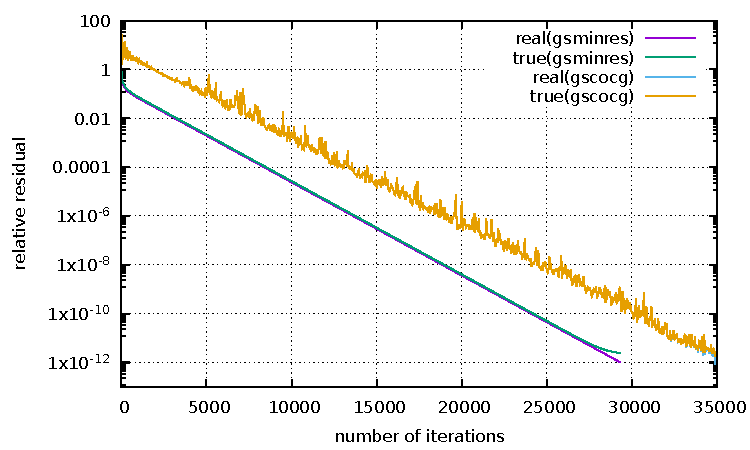
\includegraphics[scale=1.5]{./fig/compare-residual.pdf} }
			\caption{$k=1$における相対残差の比較}
			\label{fig-compare-residual}
		\end{minipage}
		\begin{minipage}[]{0.49\columnwidth}
			\centering
			\makeatletter
			\def\@captype{table}
			\makeatother
			\caption{実行時間と反復回数の比較}
			\label{table-compare-time-itrs}
			\begin{tabular}{ccc}
				\hline
						& 実行時間(秒)	& 反復回数	\\ \hline
				gsminres	& 11874		& 29342	\\
				gscocg	& 14457		& 34815	\\
				\hline
			\end{tabular}
		\end{minipage}
	\end{center}
\end{figure}

\begin{figure}[H]
	\begin{center}
		\begin{minipage}[t]{0.49\columnwidth}
			\centering
			\colorbox{white}{ 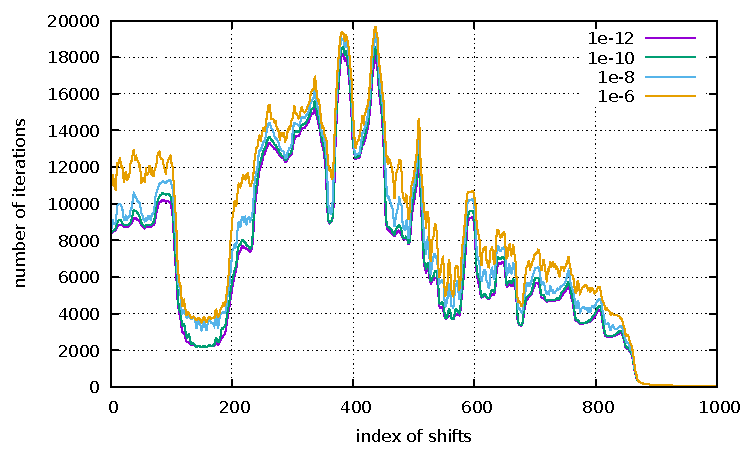
\includegraphics[scale=1.5, page=1]{./fig/compare-inner.pdf} }
			\caption{内部反復の精度と反復回数の比較}
			\label{fig-compare-inner-itr}
		\end{minipage}
		\begin{minipage}[t]{0.49\columnwidth}
			\centering
			\colorbox{white}{ \includegraphics[scale=1.5, page=2]{./fig/compare-inner.pdf} }
			\caption{内部反復の精度と真の相対残差の関係}
			\label{fig-compare-inner-res}
		\end{minipage}
	\end{center}
\end{figure}

\begin{itemize}
	\item gsminresは滑らかに残差のノルムが減少している
		\begin{itemize}
			\item 残差のノルムを最小化しているから
		\end{itemize}
	\item gsminresはアルゴリズム上での残差(real)と真の残差(true)で乖離がある
		\begin{itemize}
			\item $2$--ノルムではなく$B^{-1}$--ノルムの最小化であるから
		\end{itemize}
	\item gsminresがgscocgよりも少ない反復回数で収束し,高速である
	\item 外部反復の精度は内部反復の精度程度しかでない
\end{itemize}


\begin{comment}
% https://tex.stackexchange.com/questions/195195/import-pdf-with-white-background


\begin{itemize}
	\item gsminresは滑らかに残差が減少している\\
		\myitem 残差のノルムを最小化しているから
	\item gsminresはアルゴリズム上での残差(real)と真の残差(true)で乖離がある\\
		\myitem $2$--ノルムではなく$B^{-1}$--ノルムの最小化であるから
	\item gsminresがgscocgよりも少ない反復回数で収束し,高速
	\item 外部反復の精度は内部反復の精度程度しかでない
\end{itemize}

\textcolor{structure.fg}{\textbullet} gsminresは滑らかに残差が減少している\\
		\myitem $2$--ノルムではなく$B^{-1}$--ノルムの最小化であるから\\
\textcolor{structure.fg}{\textbullet} gsminresはアルゴリズム上での残差(real)と真の残差(true)で乖離がある\\
		\myitem $2$--ノルムではなく$B^{-1}$--ノルムの最小化であるから\\
\textcolor{structure.fg}{\textbullet} gsminresがgscocgよりも少ない反復回数で収束し,高速\\
\textcolor{structure.fg}{\textbullet} 外部反復の精度は内部反復の精度程度しかでない

\end{comment}
		\end{block}
		\begin{block}{まとめと今後の展望}
			\vspace{0.2\baselineskip}
			
\begin{itemize}
	\item 一般化シフト線形方程式に対するGeneralized shifted MINRES法を構築した
		\begin{itemize}
			\item 一般化Lanczos過程に基づき,残差の$B^{-1}$--ノルムを最小化する
			\item $A, B$がエルミート行列である場合にも適用可能である
		\end{itemize}
	\item 更なる数値実験による優位性の検証
	\item 理論的な収束特性の評価をおこなう
\end{itemize}
		\end{block}
		\begin{block}{参考文献}
			


%\setlength{\baselineskip}{40pt}
\textcolor{black}{
%\footnotesize
\fontsize{28pt}{15pt}\selectfont
\begin{thebibliography}{7}
	\vspace{-2mm}
	\bibitem{ref-SeitoH-2019}
		S.~Hiroaki, T.~Hoshi, and Y.~Yamamoto,
		 On using the shifted minimal residual method for quantum-mechanical wave packet simulation,
		JSIAM Let., \textbf{11} (2019), 13--16.
	\bibitem{ref-SogabeT-2010}
		S.~Tomohiro, T.~Hoshi, S.~-L.~Zhang, and T.~Fujiwara,
		A fast numerical method for generalized shifted linear systems with complex symmetric matrices,
		\textmc{数理解析研究所講究録}., \textbf{1719} (2010), 106--117.
	\bibitem{ref-ELSES-matrix}
		T. Hoshi, ELSES matrix library, 2019, http://www.elses.jp/matrix/. (accessed 13 Aug. 2024)
\end{thebibliography}
}


\begin{comment}

\bibliographystyle{junsrt}
\bibliography{ref}

	\bibitem{ref-SeitoH-2019}
		S.~Hiroaki, T.~Hoshi, and Y.~Yamamoto,
		\newblock On using the shifted minimal residual method for quantum-mechanical wave packet simulation,
		\newblock JSIAM Let., {\bf 11} (2019), 13--16.
	\bibitem{ref-SogabeT-2010}
		S.~Tomohiro et.al.,
		\newblock A fast numerical method for generalized shifted linear systems with complex symmetric matrices,
		\newblock 数理解析研究所講究録., {\bf 1719} (2010), 106--117.


\end{comment}

		\end{block}
	\end{column}
	\end{columns}
	\vspace{0.4\baselineskip}
	\center{第22回 計算数学研究会}
\end{frame}

\end{document}


% 参考
% https://github.com/hyoiutu/myPosterTemplate/tree/master